\section{Optimal Communication Chain over the Ideal Channel}
\textcolor{red}{[TODO: ADD MORE MATH LATER]}\par
\textcolor{red}{[TODO: MAYBE ADD HOW SOME SIMULATION PARAMETERS AFFECT THE SIMULATION (like taps for example)]}\par
\textcolor{red}{[TODO: MAKE THE AXIS NUMBER OF THE GRAPHS BIGGER]}\par

\subsection{Communication Chain}
\begin{figure}[H]
	\centering
	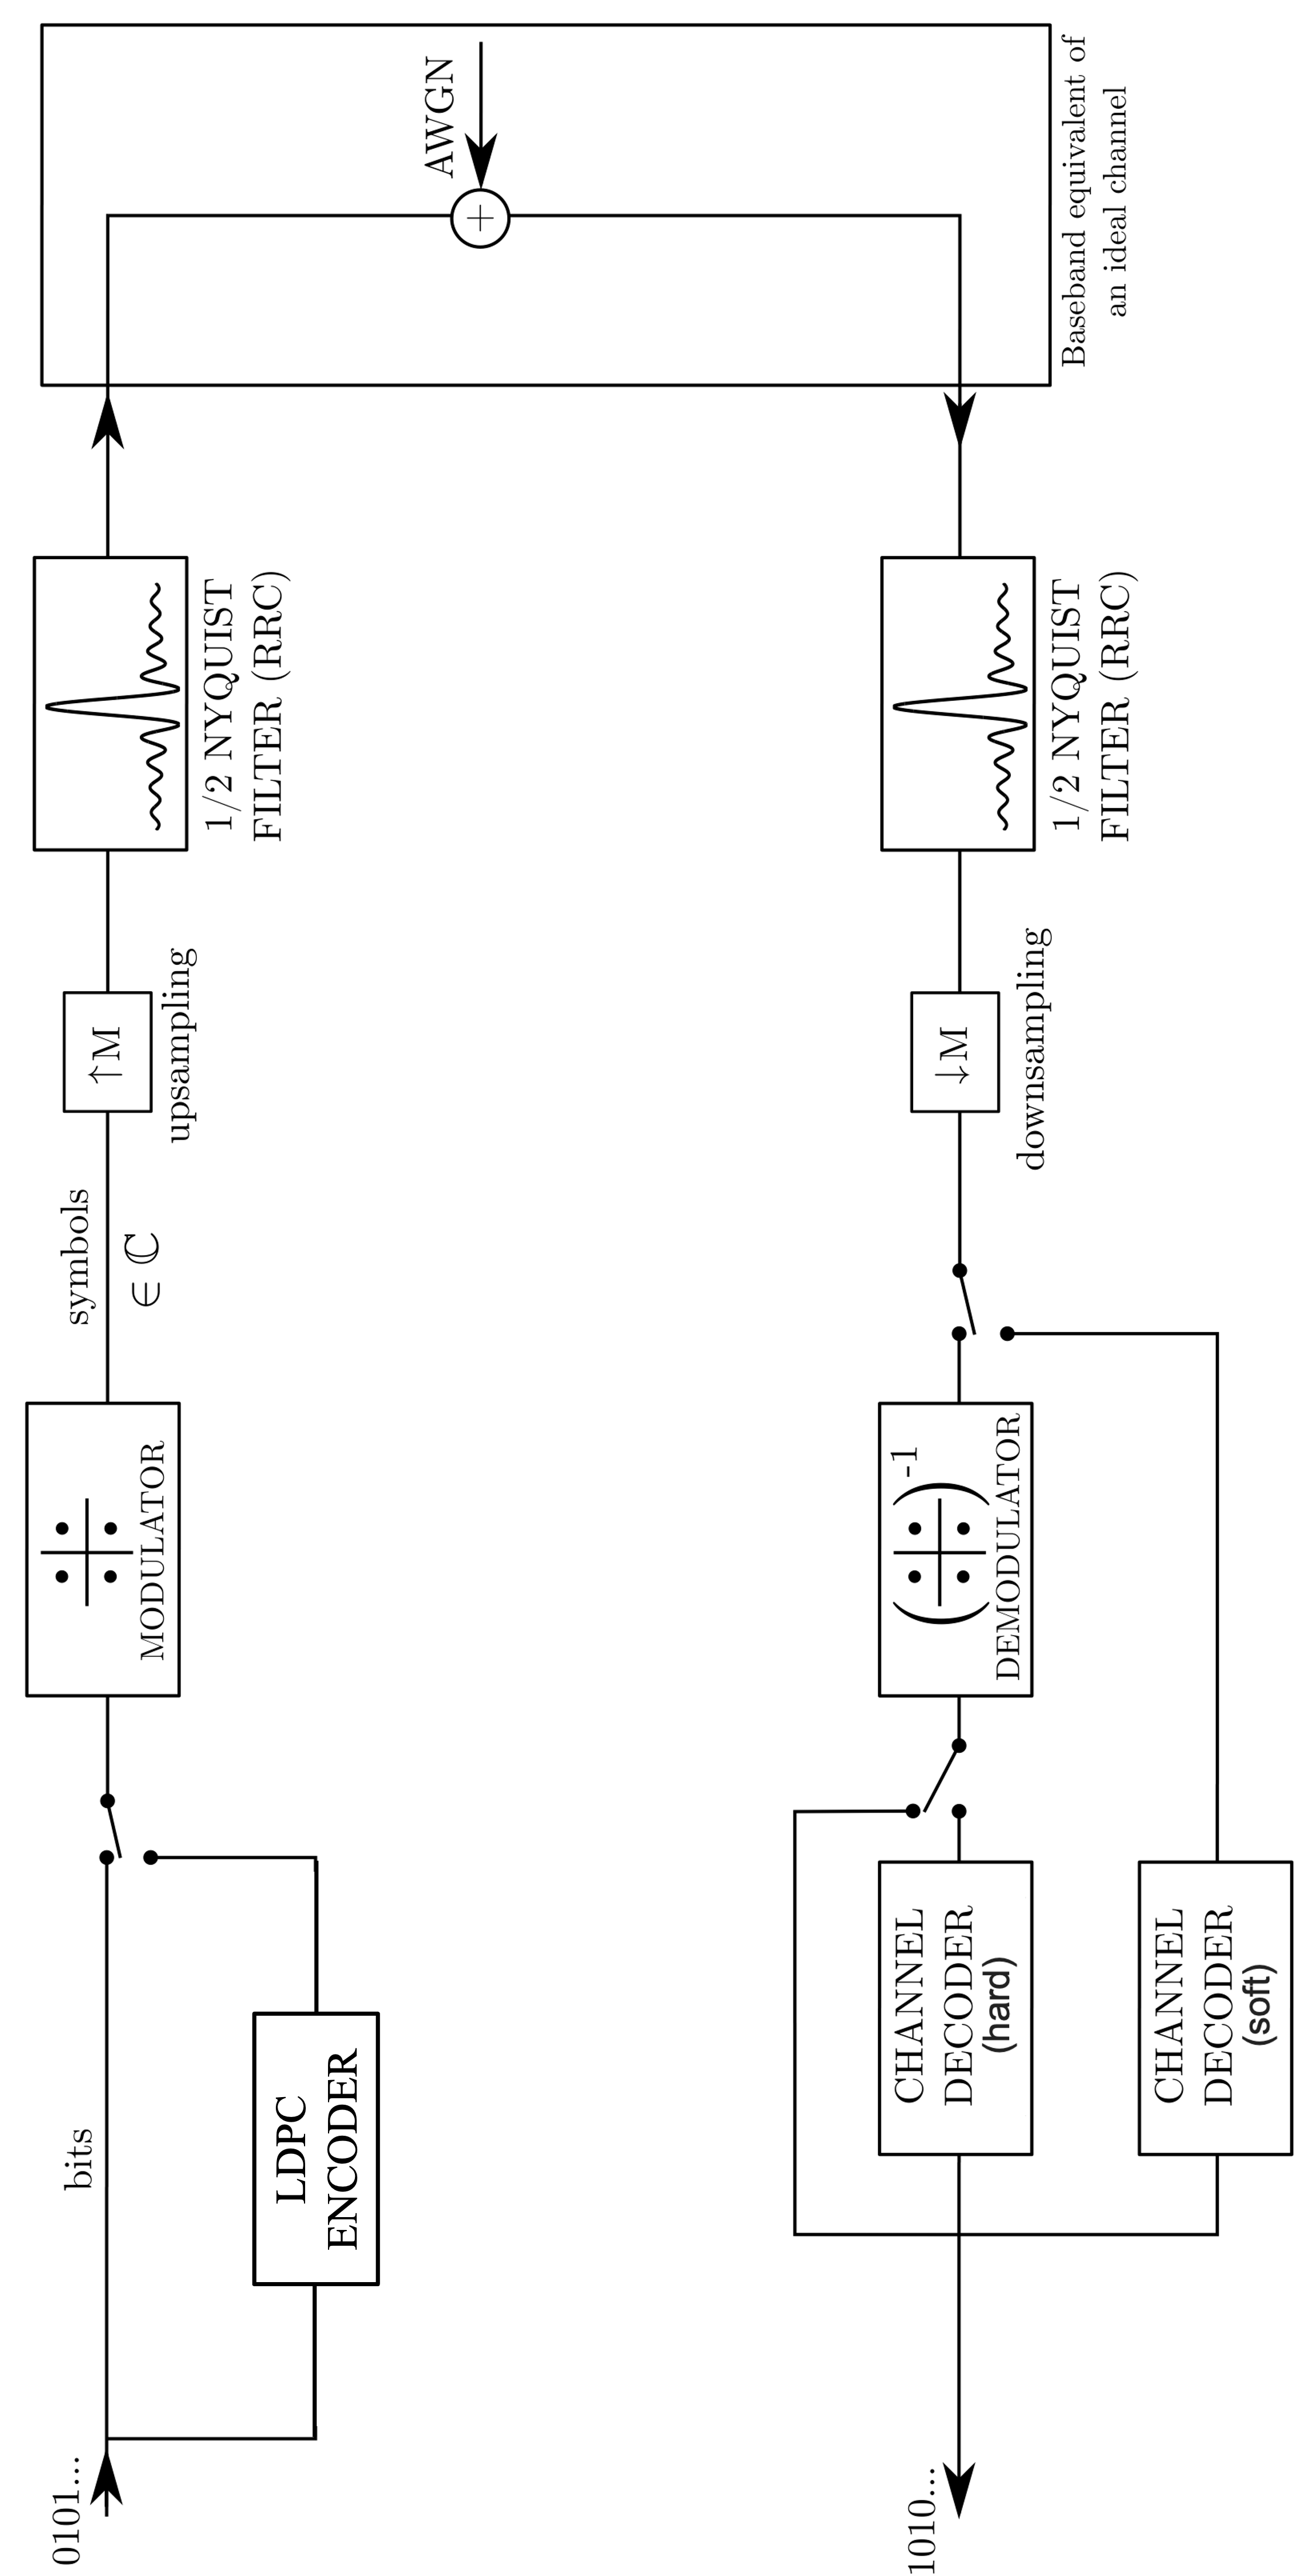
\includegraphics[angle=-90, width=0.9\linewidth]{Images/com-chain} % Ensure 'Images/com-chain' path is correct
	\caption{Block diagram of the communication system}
	\label{fig:com-chain}
\end{figure}
The communication chain depicted in Figure \ref{fig:com-chain} models the pipeline of a DVB-C transmitter and receiver at baseband. On the transmitter side, a bit-stream is generated, then mapped to complex symbols from a chosen QAM modulation. These symbols are subsequently up-sampled and shaped by a half-root Nyquist filter to limit their bandwidth. On the receiver's side, the transmitted signal is matched-filtered with the same half-root Nyquist filter to maximize the signal-to-noise ratio. The output of the matched filter is then down-sampled at the symbol instances and demapped to recover an estimate of the transmitted bit-stream.\\
In this project, the Low Density Parity Check Encoder is not implemented, and the algorithms for symbol mapping and demapping were provided.

\subsection{Bit Generation and Symbol Mapping and Demapping}
The mapping of bit-streams to complex symbols enhances spectral efficiency by allowing more bits to be transmitted per symbol over a given bandwidth. At the receiver, symbol demapping converts the noisy received symbols back into an estimated sequence of bits. This is achieved using the Maximum Likelihood (ML) criterion, which selects the constellation symbol closest to the received sample in terms of minimum Euclidean distance:

\begin{equation}
	\tilde{\underline{s}}_{m}^{ML} = \arg\min_{\underline{s}_{m}} \left(\sum_{k=1}^{K}(r_{k}-s_{mk})^{2}\right)
\end{equation}
Where:
\begin{itemize}
	\item $\tilde{\underline{s}}_{m}^{ML}$ is the estimated symbol using the ML criterion.
	\item $\underline{r} = [r_1, r_2, \dots, r_K]^T$ is the received vector after demodulation.
	\item $\underline{s}_{m} = [s_{m1}, s_{m2}, \dots, s_{mK}]^T$ is the vector representing the $m$-th possible transmitted symbol.
	\item This selection minimizes the squared Euclidean distance, which is equivalent to maximizing $\ln p(\underline{r}|\underline{s}_{m})$ for an AWGN channel, where $p(\underline{r}|\underline{s}_{m})$ is the conditional probability of receiving vector $\underline{r}$ given that symbol $\underline{s}_m$ was sent.
\end{itemize}

\subsection{Nyquist Filtering}
The sequence of complex symbols $I[k]$, after mapping, is up-sampled by a factor of $OSF > 1$ and then passed through a pulse shaping filter $g(t)$. This filtering is essential for:
\begin{enumerate}
	\item Limiting the bandwidth of the transmitted signal.
	\item Controlling interference between successive symbols.
\end{enumerate}

\subsubsection{Half-Root Nyquist Filter Design and Matched Filtering}
To achieve optimal performance in terms of ISI cancellation and maximizing the SNR at the receiver, a root-raised cosine (RRC) filter is utilized. This involves employing an RRC filter $g(t)$ at the transmitter and its matched version $g^*(-t)$ at the receiver. The convolution of these two filters, $h(t) = g(t) \otimes g^*(-t)$, forms the overall channel response. This response $h(t)$ is designed to satisfy the Nyquist criterion for zero ISI, which states that for symbols sampled at intervals $T_{symb}$:
\begin{equation}
	h(kT_{symb}) = \begin{cases}
		1 & k=0 \\
		0 & k \neq 0
	\end{cases}
\end{equation}
To design the RRC filter $g(t)$, the transfer function of a raised-cosine (RC) filter, $H(f)$, is first defined. The frequency response of the RRC filter is then $G(f) = \sqrt{H(f)}$, and its time-domain equivalent $g(t)$ is found via an inverse Fourier transform.\\
The frequency response of the RC filter, characterized by a roll-off factor $\beta = 0.2$, is given by:
\begin{equation}
	H(f) = \begin{cases}
		T_{symb} & 0 \le |f| < \frac{1-\beta}{2T_{symb}} \\ % Corrected T to T_symb
		\frac{T_{symb}}{2} \left(1 + \cos\left[\frac{\pi T_{symb}}{\beta}\left(|f| - \frac{1-\beta}{2T_{symb}}\right)\right]\right) & \frac{1-\beta}{2T_{symb}} \le |f| \le \frac{1+\beta}{2T_{symb}} \\ % Corrected T to T_symb
		0 & |f| > \frac{1+\beta}{2T_{symb}} % Corrected T to T_symb
	\end{cases}
\end{equation}

\subsubsection{Filter Properties and Inter-Symbol Interference Cancellation}
The RC filter effectively confines the signal energy within a bandwidth $B = R_{symb} (1+\beta)/2$, where $R_{symb} = 1/T_{symb}$ is the symbol rate. Figure \ref{fig:h-rc-freq} illustrates this, showing a flat passband, a roll-off region, and a stopband, restricting the signal to its allocated spectrum. For project parameters ($R_{symb} = !!!!!!!!!!$ and $\beta = 0.2$), the communication bandwidth is $B = 0.6 R_{symb}$.

\begin{figure}[H]
	\centering
	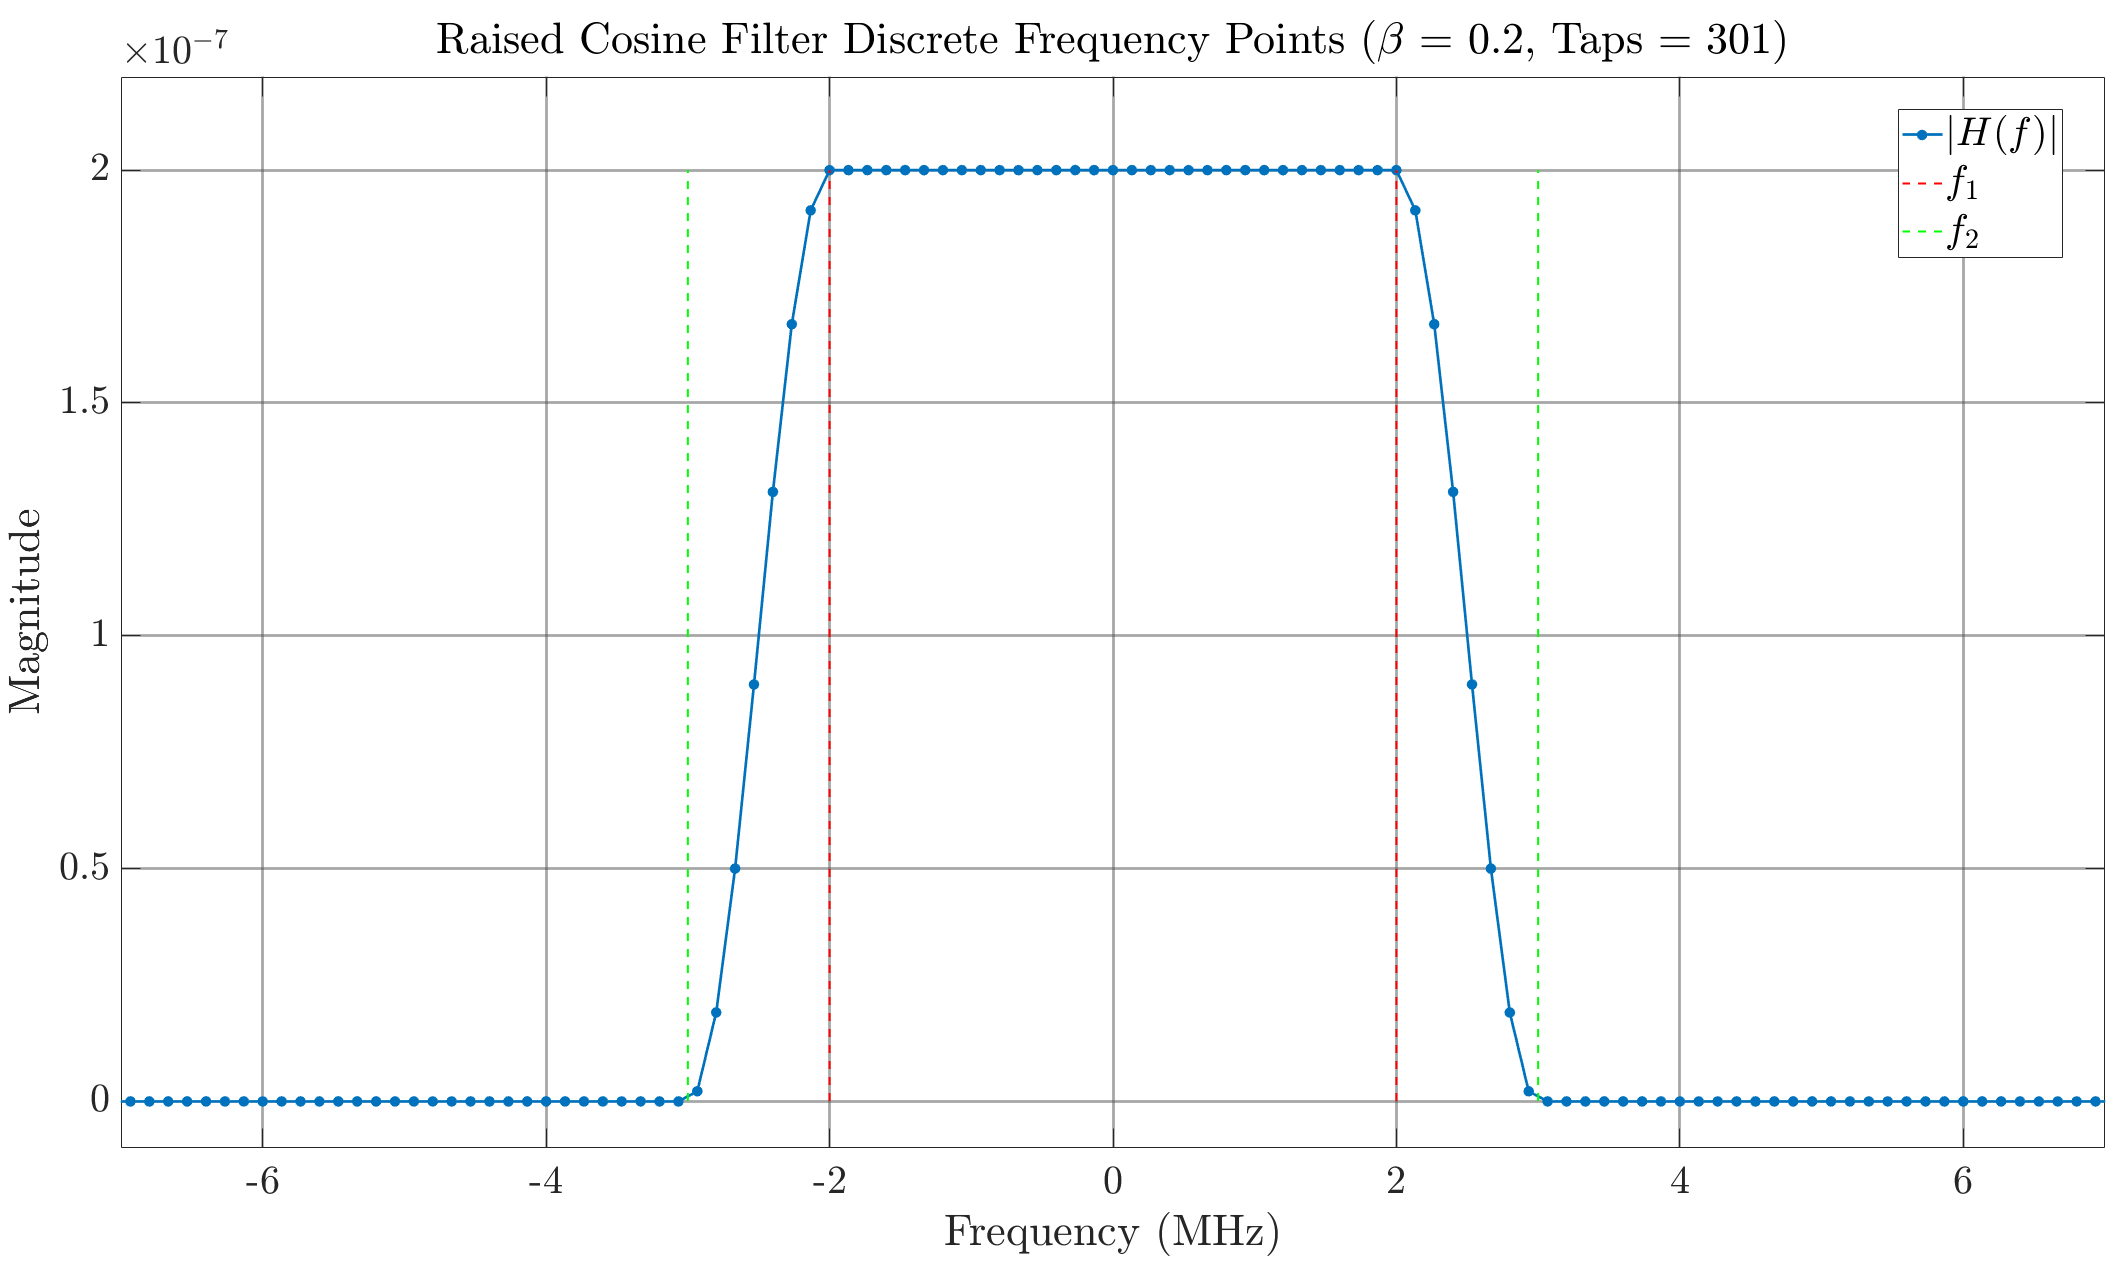
\includegraphics[width=0.9\linewidth]{Images/h-rc-freq} % Ensure 'Images/h-rc-freq' path is correct
	\caption{Raised Cosine Filter Frequency Response ($\beta = 0.2$, $taps = 301$, $OSF = 8$)}
	\label{fig:h-rc-freq}
\end{figure}

In the time domain, the impulse response of the overall RC filter $h(t)$, when sampled at the symbol rate, approximates a Dirac delta function. As shown by the stems representing $h(kT_{symb})$ in Figure \ref{fig:h-rc}, the normalized response is unity at $t=0$ and zero at $t = \pm T_{symb}, \pm 2T_{symb}, \dots$. This property ensures that at the optimal sampling instant for a given symbol, contributions from all other symbols are nullified, thereby eliminating ISI.

\begin{figure}[H]
	\centering
	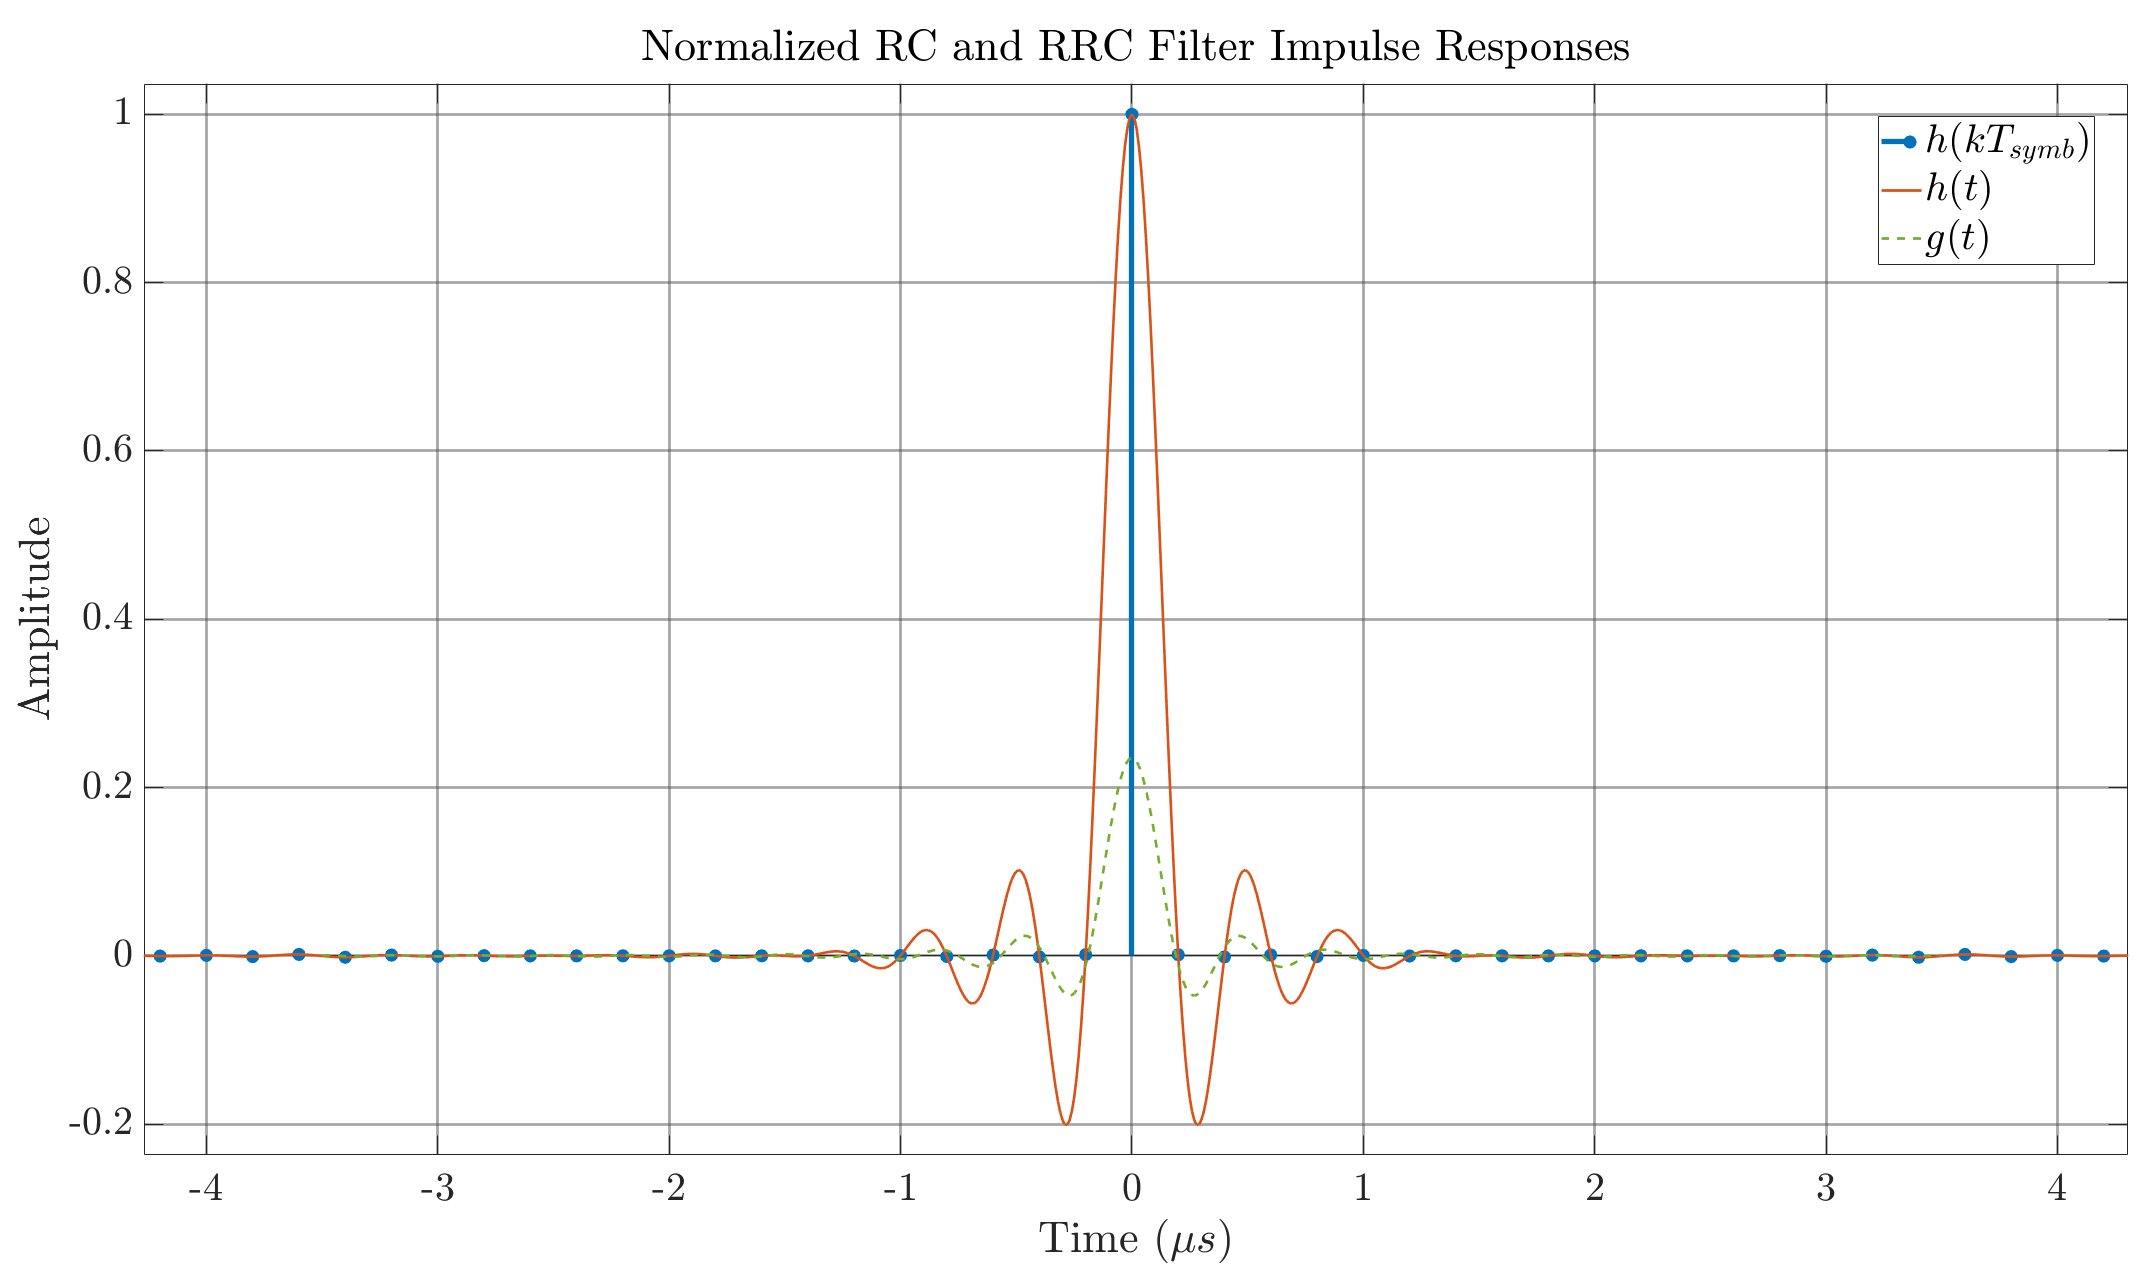
\includegraphics[width=0.9\linewidth]{Images/h-rc} % Ensure 'Images/h-rc' path is correct
	\caption{Normalized RC and RRC filter Impulse Responses, and ISI cancellation}
	\label{fig:h-rc}
\end{figure}

\subsection{Noise Addition and Performance Evaluation}
One of the factor limiting communication performance in an ideal channel is the Additive White Gaussian Noise, which represents the cumulative effect of various sources of interference and thermal noise within a communication system.\par

In the baseband equivalent model, the received signal $r(t)$ is the sum of the transmitted baseband signal $s(t)$ and the complex baseband equivalent noise $n(t)$:
\begin{equation}
    r(t) = s(t) + n(t)
\end{equation} \par
The noise $n(t)$ is a complex Gaussian random process. Its real and imaginary components are independant, each with a power spectral density of ${N_0}/{2}$ over the bandwidth of interest.\par
After matched filtering with $g(-t)$ and sampling at $t = kT_{symb}$, the $k$-th received sample $y[k]$
can be expressed as
\begin{equation}
    y[k] = (r(t) \otimes g(-t))|_{t=kT_{symb}}
\end{equation}
\par
Given that the overall response $h(t) = g(t) \otimes g(-t)$ is designed to satisfy the Nyquist criterion for zero ISI:
\begin{align}
    y[k] &= I[k]h(0) + \sum_{m \neq k} I[m]h((k-m)T_{symb}) + (n(t) \otimes g(-t))|_{t=kT_{symb}}\\
    y[k] &= I[k] + (n(t) \otimes g(-t))|_{t=kT_{symb}}\\
    y[k] &= I[k] + n_o[k]
\end{align}
where $I[k]$ is the transmitted complex symbol and $n_o[k]$ represents the noise component at the output of the sampler, given by $n_o[k] = (n(t) \otimes g(-t))|_{t=kT_{symb}}$. The noise samples $n_o[k]$ are complex Gaussian random variables. Since the input noise $n(t)$ is white and Gaussian, and the matched filtering operation is linear, $n_o[k]$ is also Gaussian. The real and imaginary components of $n_o[k]$ are independent, and each has a variance $\sigma^2 = N_0/2$ \par

The main goal of this section of the project is to evaluate the system's performance by simulating the Bit Error Rate as a function of the ratio of bit energy ($E_b$) to the one-sided power spectral density of noise ($N_0$)

To accurately simulate the system at a specific $E_b/N_0$ value, the power of the simulated noise must be correctly set relative to the signal power. The average energy per symbol $E_s$, for a given QAM constellation is calculated as:
\begin{equation}
    E_s = \text{E}\left[|I[k]|^2\right]
\end{equation}
where $\text{E}[\cdot]$ is the expectation operator. If each symbol $I[k]$ represents $b = \log_2 M$ information bits (where $M$ is the constellation size), the average energy per bit $E_b$ is:
\begin{equation}
    E_b = \frac{E_s}{b} = \frac{E_s}{\log_2 M}
\end{equation}

\par
Given a target $E_b/N_0$ value, the required $N_0$ can be determined:
\begin{equation}
    N_0 = \frac{E_b}{(E_b/N_0)_{\text{target}}}
\end{equation}

\par
The complex noise $n_o[k]$ added to each symbol $I[k]$ in the simulation is thus generated with a total variance of $N_0$, meaning that its real and imaginary components each have a variance of $N_0/2$.

The experimental BER is obtained by transmitting a large number of random bits through the simulated communication chain, adding the appropriately scaled AWGN, demapping the received symbols, and then comparing the recovered bits with the originally transmitted bits:
\begin{equation}
    \text{BER}_{\text{exp}} = \frac{\text{Number of erroneously detected bits}}{\text{Total number of transmitted bits}}
\end{equation}
The simulated BER values are then plotted against a range of $E_b/N_0$ values. These experimental results are compared against theoretical BER performance for M-QAM to validate the simulation. For square M-QAM constellations with Gray coding, the theoretical BER can be approximated by recognizing that M-QAM can be decomposed into two independent $\sqrt{M}$-PAM systems. The BER theoritical is approximated at moderate to high $E_b/N_0$ values by:
\begin{equation}
    P_b \approx \frac{4}{\log_2 M} \left(1 - \frac{1}{\sqrt{M}}\right) Q\left(\sqrt{\frac{3 (\log_2 M)^2}{M-1} \frac{E_b}{N_0}}\right)
    \label{eq:Pb_MQAM_Eb_cont}
\end{equation}
where $Q(x) = \frac{1}{\sqrt{2\pi}} \int_x^\infty e^{-u^2/2} du$ is the Q-function.

Figure \ref{fig:ber-mod_cont} illustrates the simulated BER curves for various QAM modulations, demonstrating the trade-off between spectral efficiency and power efficiency; higher-order modulations achieve higher data rates within the same bandwidth but require more power (higher $E_b/N_0$) for the same BER.

\begin{figure}[H]
    \centering
    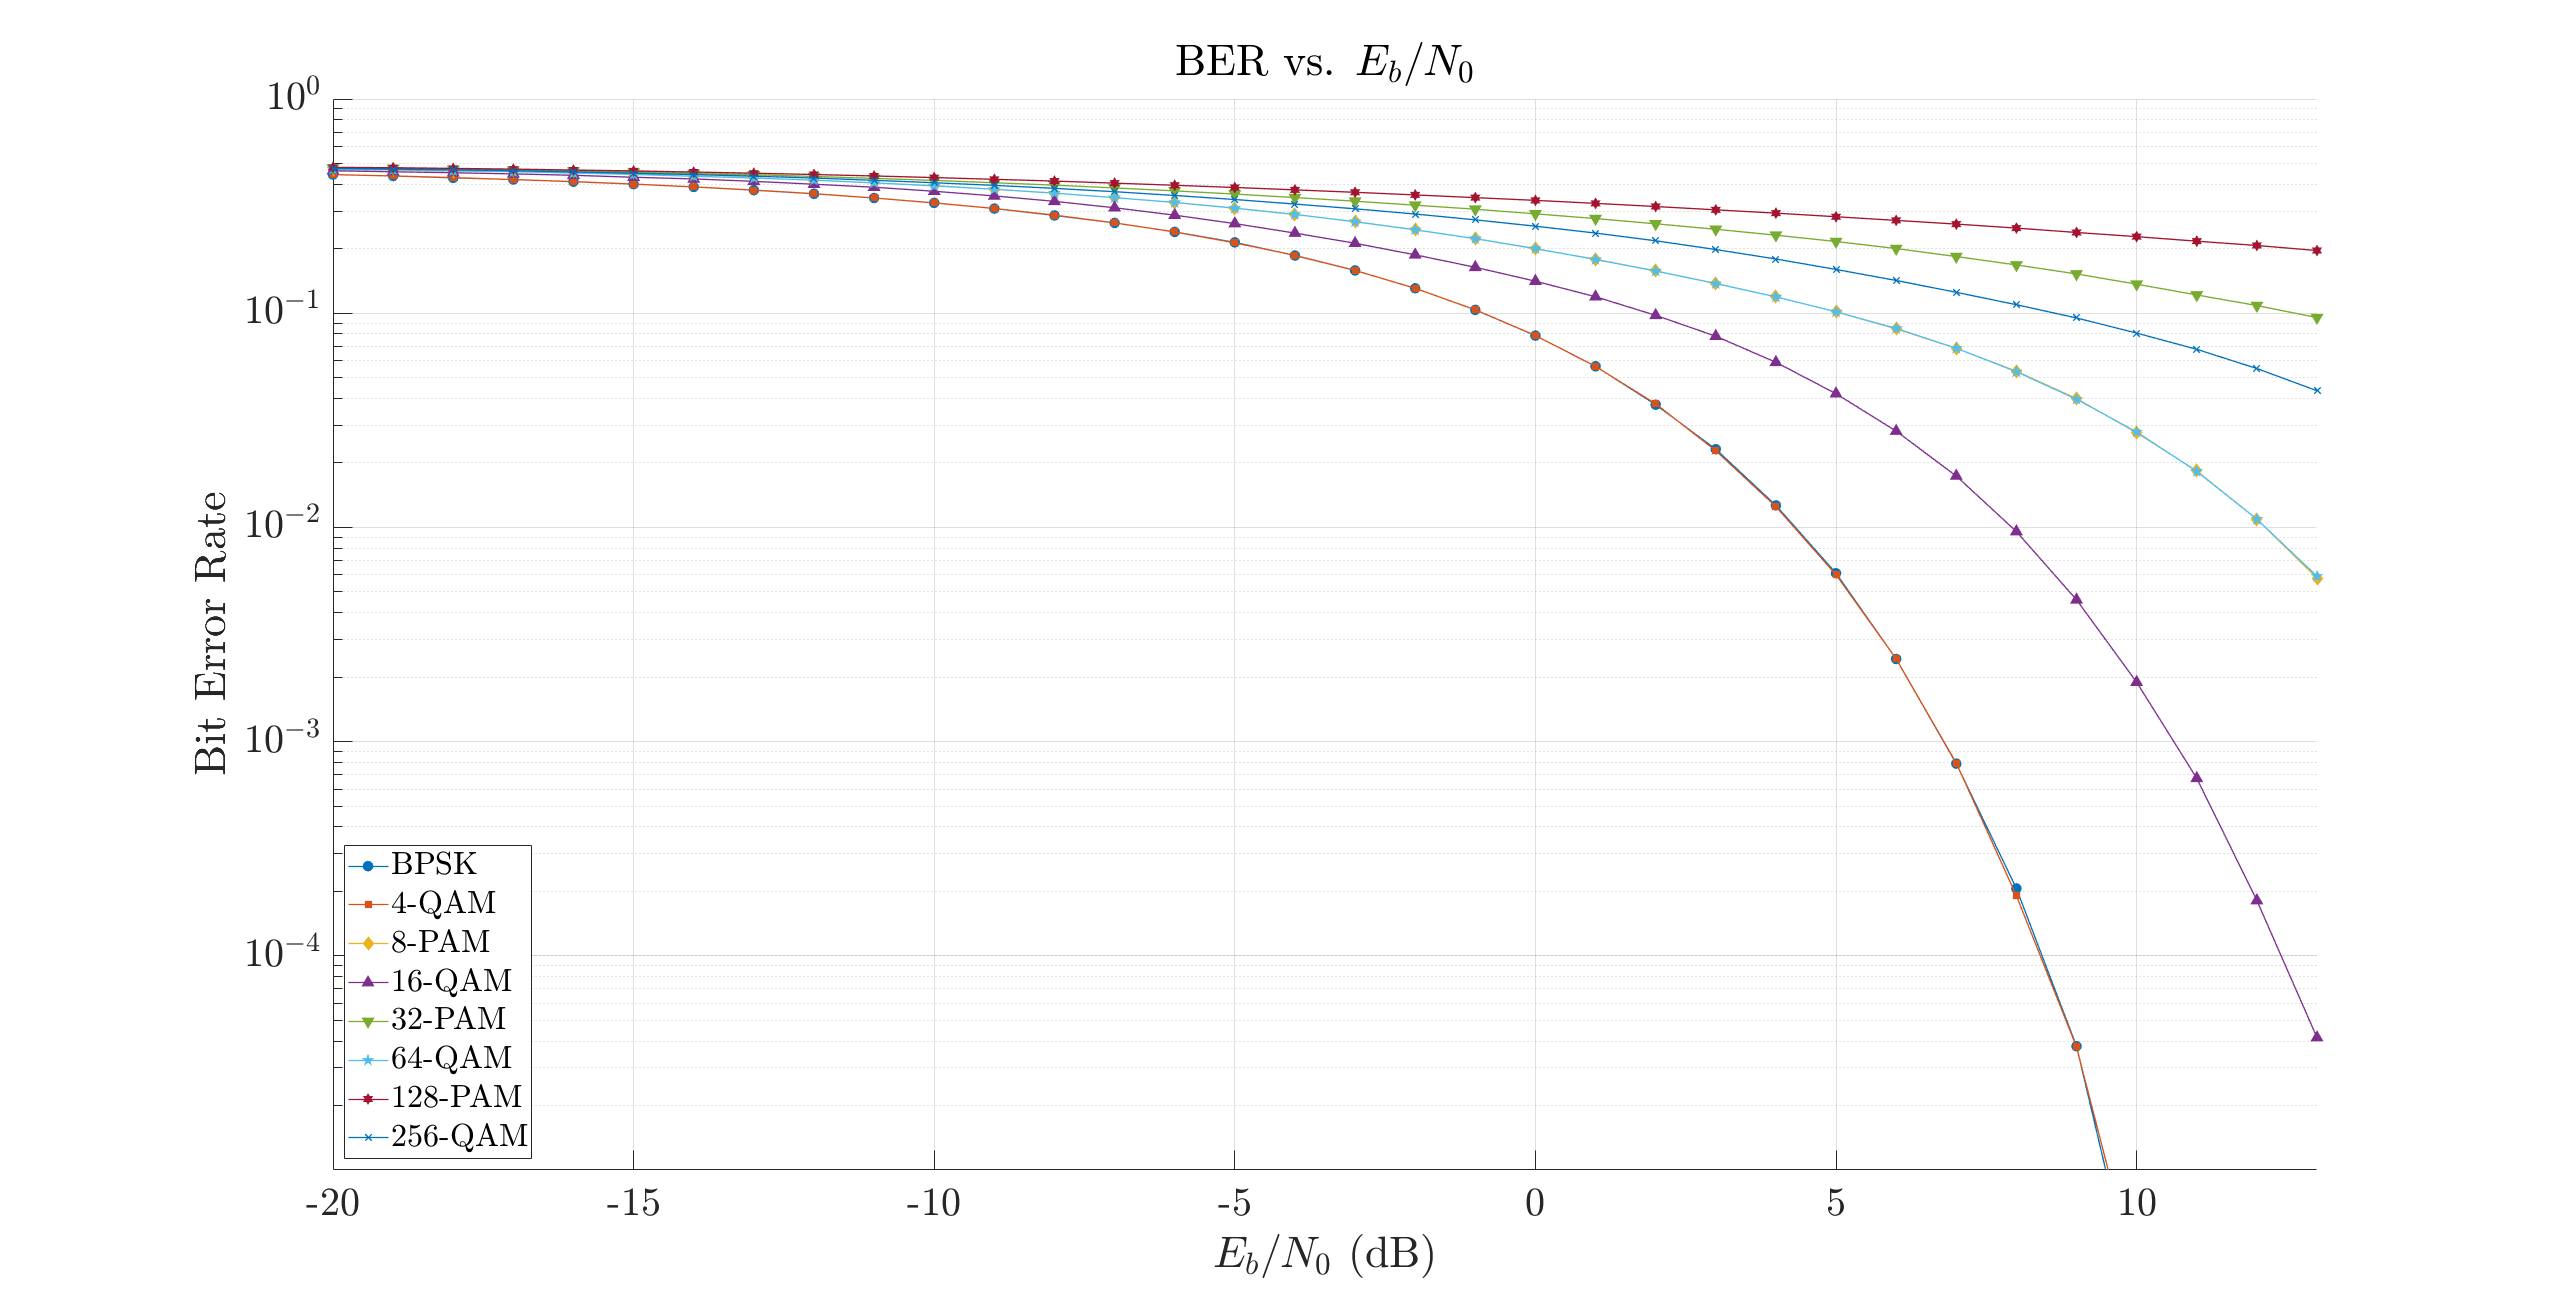
\includegraphics[width=0.9\linewidth]{Images/ber-mod.png}
    \caption{BER vs. $E_b/N_0$ for various modulation type.}
    \label{fig:ber-mod_cont}
\end{figure}

The effect of AWGN on the received signal constellation is depicted in Figure \ref{fig:constellations-noise_cont}. Figure \ref{fig:const-noisy_cont} shows conceptually how noise spreads the ideal constellation points. After matched filtering and optimal sampling, as shown in Figure \ref{fig:const-filtered-down_cont}, the signal points cluster around the ideal constellation locations, illustrating the SNR maximization by the matched filter before demapping.

\begin{figure}[H]
    \centering
    \begin{subfigure}{0.48\textwidth}
        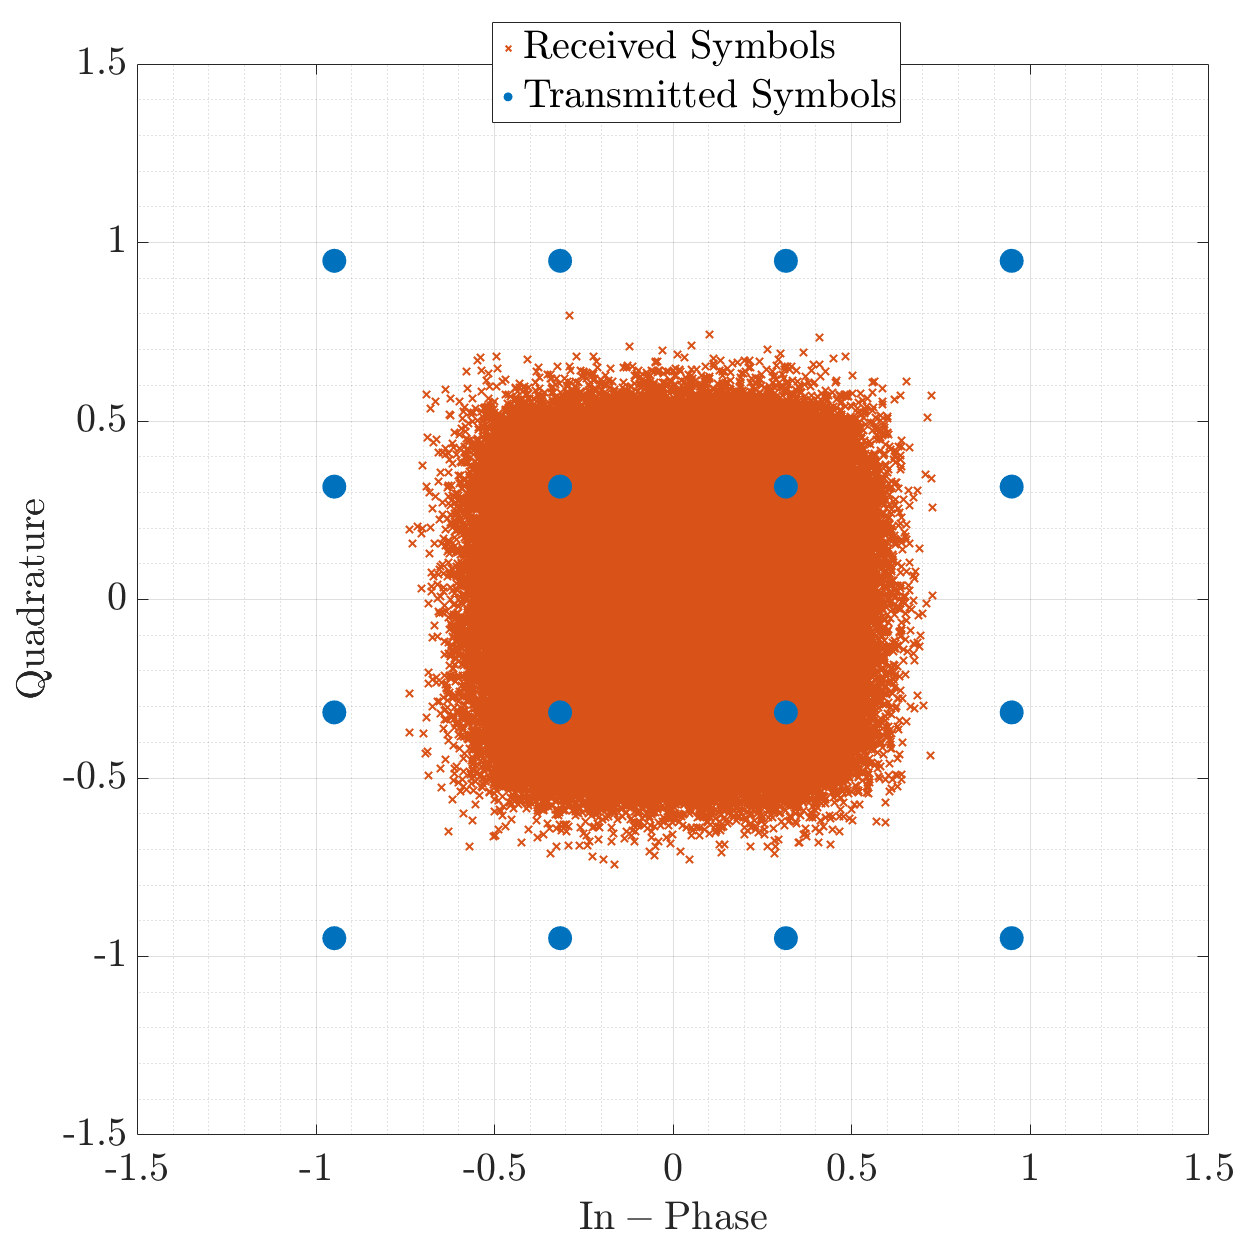
\includegraphics[width=\linewidth]{Images/const-noisy.png}
        \caption{Simulated noisy 16-QAM symbols before filtering.}
        \label{fig:const-noisy_cont}
    \end{subfigure}\hfill
    \begin{subfigure}{0.48\textwidth}
        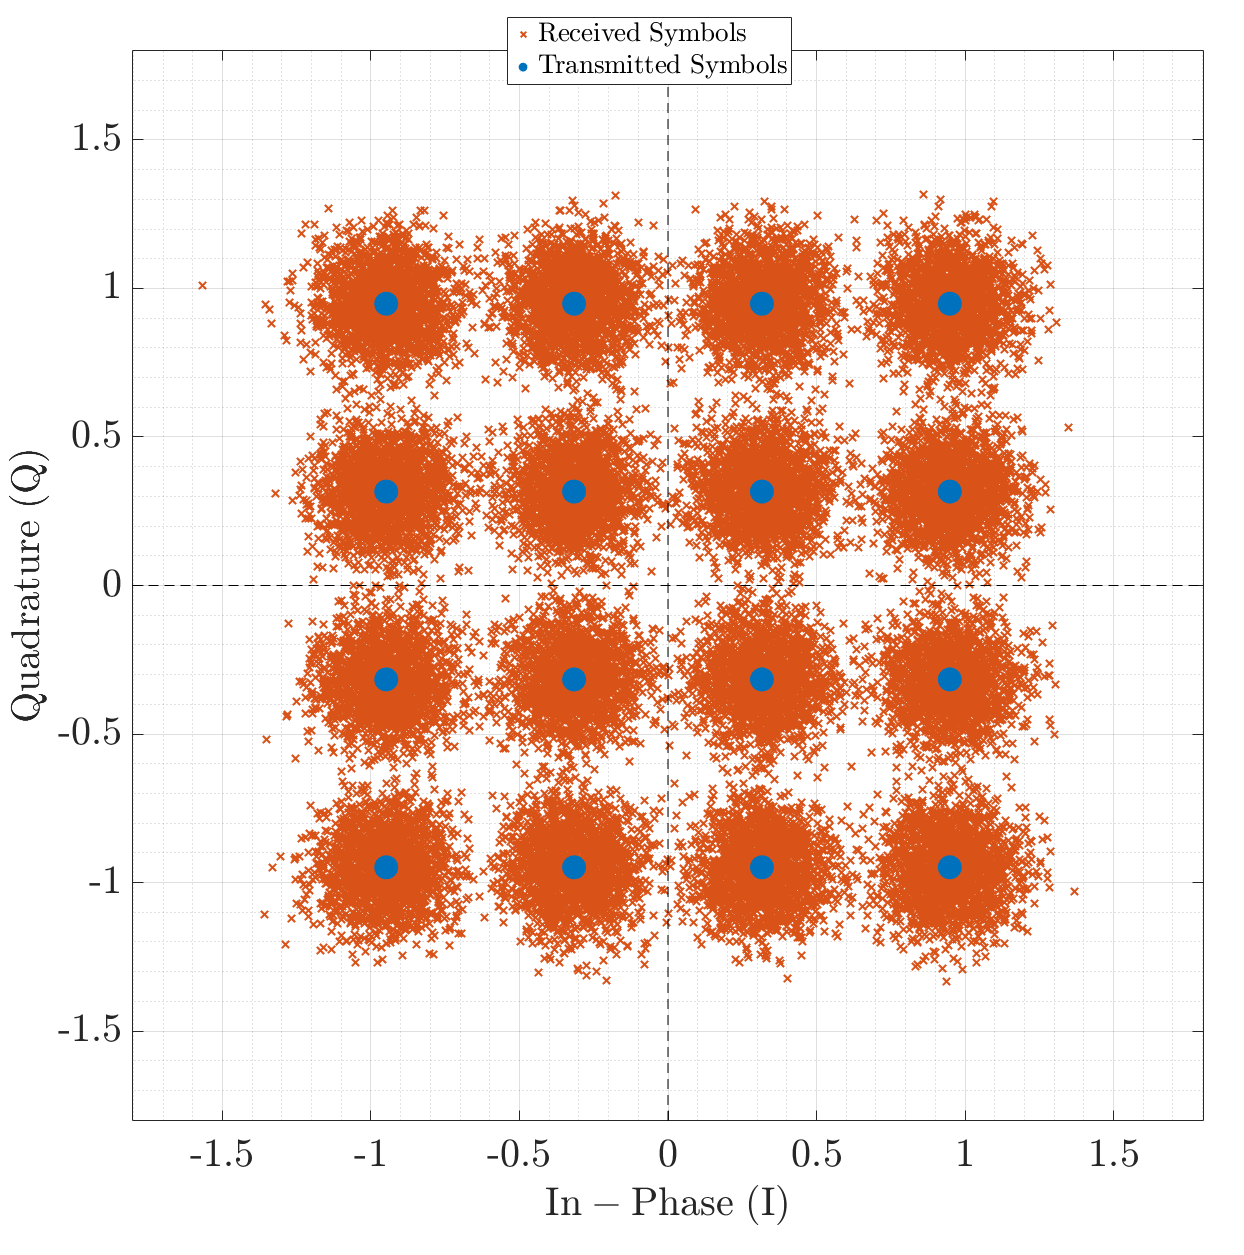
\includegraphics[width=\linewidth]{Images/const-filtered-down.png} 
        \caption{Simulated 16-QAM symbols after matched filtering and sampling.}
        \label{fig:const-filtered-down_cont}
    \end{subfigure}
    \caption{Effect of AWGN and matched filtering on a 16-QAM constellation.}
    \label{fig:constellations-noise_cont}
\end{figure}

The agreement between the simulated BER performance and the theoretical predictions based on Equation \ref{eq:Pb_MQAM_Eb_cont} serves as a verification of the correct implementation and understanding of the optimal communication chain components under AWGN conditions.


\subsection{Questions and Answers}
\textcolor{red}{[LATER]}